\documentclass[12pt,a4 paper]{report}  % To indicate fontsize, page type and document type
\renewcommand{\baselinestretch}{1.5} % To make the linespacing in the document 1.5cm
%\renewcommand{\bibname}{}  % To make title "BIBLIOGRAPHY" to "REFERENCES"
%\usepackage{amsmath,graphicx,color,geometry,fancyhdr,subfigure}
\usepackage{amsmath,epsfig,cite,graphicx,ltablex,tabularx,setspace,url,
floatflt,caption,float,comment,fancyhdr,geometry,subfigure,amssymb,color,indentfirst,booktabs,array,xspace,nomencl}
%\usepackage[caption=false,font=footnotesize]{subfig}
\DeclareMathOperator*{\esup}{argmax}
%\usepackage{amsmath,graphicx,color,geometry,subfigure}
%  'amsmath'   --   for [equation*]
%  'graphicx'    --   To include figures
%  'color'          --   To include texts with color and also with different fonts
%  'geometry'   --   To change page properties
%  'fancyhdr'    --   To make the pages look good by including special effects
%  'subfigure'   --   To include two figures in a single figure
% INCLUDE subfigure after fancyhdr since now it is not working because packages are not updated fully.

\geometry{left=1.25in,right=1in}
\geometry{top=1.1in,bottom=1in}       % page geometry

\setcounter{secnumdepth}{3}%
% to get subsubsections numbered
\setcounter{tocdepth}{3}%
% to get subsubsections in the table of contents

% Project Details
\newcommand{\projectName}{DaxOS\xspace}

\newcommand{\firstAuthor}{Nihal Narayan\xspace}
\newcommand{\firstAuthorRegNo}{MBT17CS081\xspace}

\newcommand{\secondAuthor}{Antony S. Chirayil\xspace}
\newcommand{\secondAuthorRegNo}{MBT17CS023\xspace}

\newcommand{\thirdAuthor}{Mathew Koshy\xspace}
\newcommand{\thirdAuthorRegNo}{MBT17CS068\xspace}

\newcommand{\fourthAuthor}{R Midhun Suresh\xspace}
\newcommand{\fourthAuthorRegNo}{MBT17CS095\xspace}

\begin{document}  % actual document beginning
\renewcommand\bibname{REFERENCES}

%-----COVER PAGE-----%
\begin{titlepage}
\begin{center}
{\Large\sf \textbf{\textcolor[rgb]{0,0,0}{{DaxOS}}}}\\[5ex]
\vspace{0.3 cm}
A PROJECT REPORT\\
submitted by

{\small \textcolor[rgb]{0,0,0}{\emph{By}} \\[1ex]

{\sf \sf {\textcolor[rgb]{0,0,0}{Nihal Narayan (MBT17CSXX) \\ Antony S. Chirayil (MBT17CSXX) \\ Mathew Koshy (MBT17CSXX) 
			\\ R Midhun Suresh (MBT17CS095)}}} \\% Enter the name of author
\vspace{0.5 cm}
to
\\
\vspace{0.5 cm}
\textbf{the APJ Abdul Kalam Technological University \\
	in partial fulfillment of the requirements for the award of the Degree }\\
\vspace{0.8 cm}
of
\\
 
%\vspace{0.8 cm}
%\\
%\textbf{FACULTY OF COMPUTER SCIENCE AND ENGINEERING}

%\textit{\textcolor[rgb]{0,0,0}{{In partial fulfillment of the requirements \\ for the award of the degree\\ of} \\}}
\textbf{BACHELOR OF TECHNOLOGY}}
\\
IN 
\\
\textit{COMPUTER SCIENCE AND ENGINEERING}
\\
    \textbf{ May, 2019}
% DEPT: Enter the name of Department,  SPECIALIZATION: Enter the specialization, 
\vspace{0.2 cm} \\[2ex]

 \begin{figure}[ht]
 \begin{center}
\resizebox{2in}{!}{
\includegraphics{mbcetlogo-eps-converted-to}}
 \end{center}
 \end{figure}

{\sf \textbf{\textcolor[rgb]{0,0,0}{DEPARTMENT OF COMPUTER SCIENCE AND ENGINEEERING}}}\\[0.5ex]
{\sf {\textcolor[rgb]{0,0,0}{MAR BASELIOS COLLEGE OF ENGINEERING \& TECHNOLOGY}}}\\[0.4ex]
Bethany Hills, Nalanchira\\
{\sf \textcolor[rgb]{0,0,0}{Thiruvananthapuram 15}}\\[0.5ex]

\end{center}
\end{titlepage}


%-----COVER PAGE-----%

%-----CERTIFICATE-----%
\thispagestyle{empty}

\setlength{\headsep}{0.4in}
\begin{center}

{\sf \textbf{\textcolor[rgb]{0,0,0}{DEPARTMENT OF COMPUTER SCIENCE AND ENGINEERING}}}\\[0.5ex]
{\sf{\textcolor [rgb]{0,0,0} MAR BASELIOS COLLEGE OF ENGINEERING \& TECHNOLOGY}}\\[0.4ex]
Nalanchira, Thiruvananthapuram.



\end{center}


\vspace{0.15cm}
 \begin{figure}[!h]
 \begin{center}
\resizebox{2in}{!}{
\includegraphics{mbcetlogo-eps-converted-to}}
 \end{center}
 \end{figure}
\vspace{0.02cm}

\begin{center}
\textcolor[rgb]{0,0,0}{\textbf{\underline{CERTIFICATE}}} \\[1ex]
\end{center}
\par

\emph{
\textit{{This is to certify that the report entitled \textbf{\projectName}  submitted by \textbf{\firstAuthor(\firstAuthorRegNo)},
		\textbf{\secondAuthor(\secondAuthorRegNo)},
		\textbf{\thirdAuthor \\ (\thirdAuthorRegNo)},
		\textbf{\fourthAuthor(\fourthAuthorRegNo)}
		 to the APJ Abdul Kalam Technological University in partial fulfillment of the
		requirements for the award of the Degree of {Bachelor of Technology} in {Computer Science and Engineering and Technology} is a bonafide record of the project work carried out by him/her under my/our guidance and supervision.This report in any form has not been submitted to any other University or Institute for any purpose}}} 



\vspace{3.0 cm}



\begin{tabular*}{\textwidth}{c @{\extracolsep{\fill}} ccc}
	\textbf{Ms. Gayathri K. S.} & 	\textbf{Mr. V. S. Shibu} & 	\textbf{Dr. Tessy Mathew} \\ 
	Project Coordinator & Guide & Head of the Department 
\end{tabular*}


\vspace{2.0 cm}

\begin{flushleft}
\textit{\textbf{Place: Thiruvananthapuram}} \\
\textit{\textbf{Date: 12/01/2021}}	
\end{flushleft}






%-----CERTIFICATE-----%

\pagenumbering{roman}   % to get page numbers for initial pages in terms of roman numbers
%-----ACKNOWLEDGEMENTS-----%
% Thesis - Abstract
\chapter*{\centering Acknowledgement}

\begin{flushleft}
	 We would like to take this opportunity to extend our sincere gratitude to \textbf{Mr. Shibu VS} for guiding us through the process of this project.
	 We would also like to thank the seminar coordinator, \textbf{Mrs. Gayathri KS}, for providing us with this opportunity which has allowed us to explore a domain which would otherwise be beyond the confines of our academic course.
\end{flushleft}

















%-----ACKNOWLEDGEMENTS-----%

%-----ABSTRACT-----%
% Thesis - Abstract
\section*{\centering ABSTRACT}

\indent {
Every computer science enthusiast is proficient in their operating system of choice. They may
even know its underlying working from an old operating system course they took in college.
However, it is usually the case that their knowledge and understanding is limited to theory and
writing low-level system code is often considered an insurmountable challenge.
This project hopes to change this attitude by developing a minimal yet functional 32-bit
operating system that can be used in conjunction with theoretical teaching to promote and
introduce systems programming. A minimal kernel guarantees easier to read source code (as
opposed to the 27 million SLOC Linux kernel) and provides a gentler introduction to kernel
development.
The kernel will include a full keyboard and mouse driver and will have support for VGA
text-mode and graphics. It will also contain a limited libc implementation with a streamlined
build process.
Additionally, this project will serve as an illustration for good development practices (code
reuse, clean architecture, unit testing).
The 32-bit kernel will be written in C with a little of assembly for the
truly low-level aspects. 
}

%-----ABSTRACT-----%

\tableofcontents

\clearpage
\addcontentsline{toc}{chapter}{List of Figures}
\listoffigures

\clearpage
\addcontentsline{toc}{chapter}{Nomenclature}
\section*{\centering Nomenclature}
\vspace{1.5 cm}

\begin{flushleft}
	

$GDT$   \hspace{1.0 cm} Global Descriptor Table\\
$IDT$   \hspace{1.0 cm} Interrupt Descriptor Table\\
$ISR$   \hspace{1.0 cm} Interrupt Service Routine\\
$VGA$   \hspace{1.0 cm} Video Graphics Array\\
$APM$   \hspace{1.0 cm} Advanced Power Management\\



\end{flushleft}
\newpage
\pagenumbering{arabic}
\pagestyle{fancy}                       % Sets fancy header and footer
\fancyfoot{}                            % Delete current footer settings
\fancyhead{}                            % Delete current footer settings
\rhead{DaxOS Design Report}		% Write your thesis topic here
\lfoot{Dept: of {Computer Science and Engineering}}
\rfoot{ \thepage}
\renewcommand{\headrulewidth}{0.4pt}
\renewcommand{\footrulewidth}{0.4pt}
\renewcommand{\pagenumbering}{} 

\chapter{Introduction}\label{chapter:Introduction}


\indent{
The Kernel is the fundamental interconnect between hardware and software of a computer system. 
Writing a kernel (kernel programming) is considered to be a difficult endeavor because development has to start from a bare metal state. 
DAX OS is a minimal 32-bit hobbyist operating system that can be used to provide a gentle introduction to students who wish to explore the domain of systems programming.

The project is open source and licensed under GNU General Public License v3.0 to ensure unrestricted access and complete transparency. 
DAX OS comes with a terminal driver, keyboard and mouse driver and basic memory management.
The project also uses appropriate development practises such as unit-testing and version control.}

Some key facts about this project are:
\begin{itemize}
	\item Source code is hosted at \url{https://github.com/DaxKernel/OS}.
	\item About 2500 lines of code only
	\item 32-bit
	\item Low resource consumption
\end{itemize}

\newpage
\section{Objectives}\label{section:Objectives}
We propose to build a 32-bit kernel that has the following functionality:
\begin{enumerate}
	
	\item \textbf{Keyboard Driver} \\
	Dax-OS includes a fully functional PS/2 keyboard driver. The PS/2 keyboard driver will convert scan-codes generated when the user presses a key on the keyboard to an integer character code. It must be noted that all keyboards practically used in modern day utilize the USB standard. We stick with the PS/2 protocol because the USB protocol is massive and difficult to implement. However there are practically no disadvantages from such a decision because most motherboards will emulate USB keyboards as PS/2 keyboards.
	
	\item \textbf{Terminal Display Driver} \\
	DaxOS is a terminal based operating system i.e it does not support windowing.
	The display support will be implemented using VGA text-mode and real-mode.
	It will later be re-implemented in Graphics.
	
	\item \textbf{Interrupts}  \\
	DaxOS makes heavy use of interrupts for device drivers. It also uses interrupts for handling CPU exceptions. 

	\item \textbf{Memory Management} \\
	DaxOS uses a flat memory model.
	Since it is an 32-bit operating system, it will support at most 4GB of addressable memory. 
	A custom memory allocator has also be implemented.

	\item \textbf{Graphics Support} \\
	DaxOS will provide graphics capability using VESA mode. The supported resolution is 1280x720. 

	\item \textbf{Font Rendering} \\
	With graphics support, the vga text-mode based terminal driver is depreciated in favor of the higher resolution VESA mode.
	Font rendering needed for this scenario is also available.

	\item \textbf{Image Rendering} \\
	DaxOs will natively support rendering images in TGA format.
\end{enumerate}

\section{Limitations} \label{section:Limitations}
Some functionality DaxOS does not implement are:
\begin{itemize}
	\item Process Management
	\item GUI
	\item Paging
\end{itemize}

\section{Technology Stack} \label{section:Technology Stack}
The bulk of the operating system is written in the C programming language.
Certain functionality such as writing data to ports and loading tables (IDT, GDT) are implemented using either GCC inline assembly or using normal x86 assembly.

The project uses the GCC cross-compiler \& binutils to target the generic i686 platform; which is a generic 32-bit Intel P6 architecture.
The GNU Assembler and Linker are also used. The assembly syntax style used is AT\&T.

The entire compilation process is driven using GNU Make which uses Makefiles to build the project.
The compilation is initiated using BASH shell scripts.
The kernel is tested using the qemu-i386 emulator and is developed on a stable Xubuntu distribution. 

DAX OS uses git as its version control system of choice.
The git repository is uploaded on Github and every new feature is developed on its own separate branch.
Team communication and coordination are actualized using discord with Github integration enabled.



% !TeX spellcheck = en_GB
\graphicspath{ {./diagrams/} }
\chapter{Design Diagrams}\label{chapter:Design Diagrams}

\section{Use-case diagram}

\begin{flushleft}
	The use case diagram illustrates how the user interacts with the operating system. There is a total of three interactions between user and the operating system in this case.
	The first interaction that the user initiates is the boot process.\\ 
	This involves:
\end{flushleft}


\begin{enumerate}

	\item \textbf{Setting up interrupts}
	\begin{flushleft}
		The concept behind interrupts is that when a piece of hardware or software wants to
		interrupt the CPU to do something important, an interrupt is raised. The CPU
		executes a program called the ISR (Interrupt Service Routine) and returns back to
		what is was doing before.
	\end{flushleft}

	\item \textbf{Loading VGA driver}
	\begin{flushleft}
		Using VGA to print text to the screen is quite simple and is achieved by using
		VGA text-mode. The user can directly write to the video memory located at
		address 0xB8000. Each character that is to be printed requires a two-byte
		representation:
		1 byte, called the code-point is used to represent the character in ASCII.
		1 byte, is used to set the background and foreground colors. There are 16
		colors that can be used.
		In VGA text-mode a maximum of 80x25 characters can be printed on the
		screen at a time.
	\end{flushleft}

	\item \textbf{Load keyboard driver}
	\begin{flushleft}
		The keyboard driver uses the PS/2 interface to enable communication between the keyboard and the computer. When a key is pressed 
		on the keyboard, the PIC raises IRQ1. This triggers an ISR which on execution will store the pressed key on a circular buffer.
		The data from the circular buffer is read by primitives from the C standard library such as scanf in stdio. The data from keyboard is
		read from port 0x60 using inline assembly function \textbf{inportb()} defined in io.c file.
	\end{flushleft}
\end{enumerate}

\begin{flushleft}
The second interaction involves the user issuing a command to the terminal. \\
The command may require dynamic memory to be allocated. Dynamic memory is
allocated by implementing the malloc C function. The malloc function acts as a
wrapper around the kernels memory manager. This needs paging and virtual
memory to be enabled.\\
The final and last interaction between the user and the system is the shutdown
sequence. This can be implemented by supporting Intel's ACPI protocol or the now
depreciated APM protocol. These protocols control the amount of power each device
is given. Additionally shutting down specific emulators by writing data to specific
ports can be done.

\end{flushleft}




\begin{figure}[h!]
	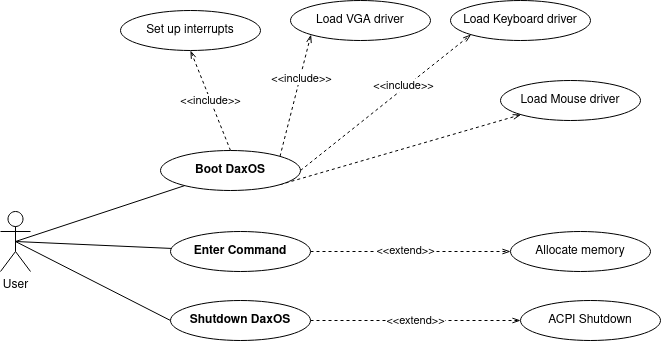
\includegraphics[width=\textwidth,height=\textheight,keepaspectratio]{use_case}
	\caption{Use Case Diagram}
\end{figure}

\pagebreak

\section{Activity Diagram}

\begin{flushleft}
	The activity diagram illustrates the shell scripts that are used to build and compile the kernel.
	
	The most important script here is the \textbf{build.sh} shell script which dives the make
	program to compile our source code. The build script relies further on two other shell
	scripts:
	\begin{enumerate}
		\item \textbf{headers.sh} script
		\begin{flushleft}
			Since in this project a version of C standard library is implemented the compilation of
			kernel is done by instructing the GCC cross-compiler to look for system headers in
			the SYSROOT directory. This script compiles the custom C std-lib into an archive
			named libk.a and places it in the SYSROOT/usr/lib directory.
			Also it copies all the .h header files into SYSROOT/usr/include directory. Now
			compiling the kernel is done by passing the --sysroot=SYSROOT parameter.
		\end{flushleft}
	
		\item \textbf{config.sh} script
		\begin{flushleft}
			This script sets up all the environment variables used by GNU Make.This allows the
			user to easily change the core aspects and tooling used in the projects later. For
			example, we could change the compiler from GCC to CLANG by simply changing
			the environment variable CC to CLANG. Likewise SYSROOT directory can be
			changed by changing a single variable.
			Once these two scripts are executed the build script runs the make-install command
			on each of the folder directory. It copies the output DaxOS.kernel file into the boot
			directory.
		\end{flushleft}
	
	\end{enumerate}

	The \textbf{iso.sh} script builds a bootable .iso image file from our kernel. It first calls the
	previously described build script and then produced an iso file by using the grub-
	mkrescue program. This iso file can be loaded into any emulator to run the operating
	system. The iso files are built into the isodir directory.
	
	\pagebreak
	The \textbf{clean.sh} script removes all the build artifacts from the compilation. Build artifacts
	are files that are produced by the compilation process that can always be
	reproduced by the compiler. Since it can be reproduced it is usually removed to
	maintain a clean project structure.
	
	There are three kinds of build artifacts:
	\begin{enumerate}
		\item  \textbf{Object files} - .o files
		\item  \textbf{Make dependencies} - .d files
		\item  \textbf{Unwanted directories} - sysroot, isodir
	\end{enumerate}

	The clean script works by executing the make clean commands in each of the
	project directories.The make clean commands use the rm bash command to delete
	the build artifacts.
	
	\vspace{1.5 cm}
	
	The last script is the \textbf{create-bootable-usb.sh} script. This script
	creates a bootable USB of the operating system. It needs sudo permission because it accesses the
	UNIX block file of the USB device. This of the form /dev/sda or something similar. 
	This script formats the USB device and copies the kernel along with the GRUB bootloader into the USB device. 
	Therefore there is a chance that the data in the USB device can be destroyed if the user is not careful.
	To prevent this a safety check that checks if the device has more than 10 GB capacity is done. If this
	is true we do not format the device and exits with error. If the capacity is less than 10GB, the USB is made bootable.
	

	
\end{flushleft}

\begin{figure}[h!]
	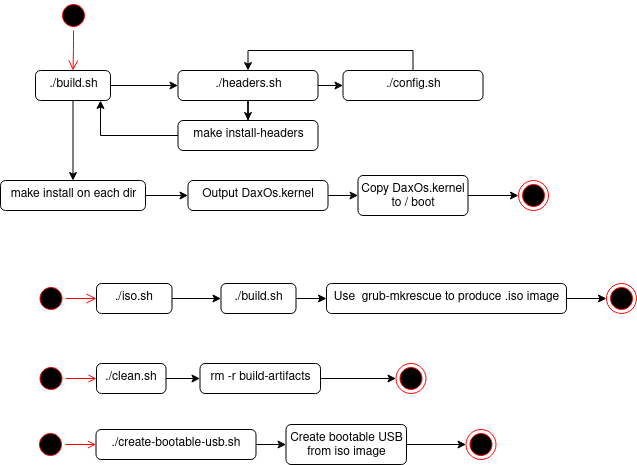
\includegraphics[width=\textwidth,height=\textheight,keepaspectratio]{activity}
	\caption{Activity Diagram}
\end{figure}

\clearpage

\section{Sequence Diagram}

\subsection{Keyboard Driver}
\begin{flushleft}
	This diagram illustrates the time dependent and sequential interaction between the
	user, the OS and the keyboard driver.
	During boot, the Operating System initializes the keyboard driver.
	This involves:
	\begin{enumerate}
		\item \textbf{Self Test}
		\begin{enumerate}
			\item The keyboard device is disabled by sending command 0xAD and 0xA7 to
			the PS/2 controller.
			\item The PS/2 controller's output buffer is flushed by reading from port 0x60.
			\item Initiate the PS/2 controller self test by sending command 0xAA to it. A
			response of 0x55 indicates success.
			\item Enable the keyboard device by sending commands 0xAE and 0xA8 to the
			PS/2 controller.
			\item Reset the device by sending 0xFF to the keyboard.
			\item Set the LED states by sending appropriate commands.
		\end{enumerate}
		\item \textbf{Handling Keypress}
		
		When the user presses a key the keyboard device initiates an interrupt. This done by
		activating IRQ1 which is the standard interrupt line used by keyboards. In response
		to this interrupt, the CPU executes an ISR which updates a buffer with the read
		characters. The I/O functions in stdio.h like scanf will read from this buffer to perform
		the necessary computation and show the results back to the user.
		
	\end{enumerate}
\end{flushleft}
\begin{figure}[h!]
	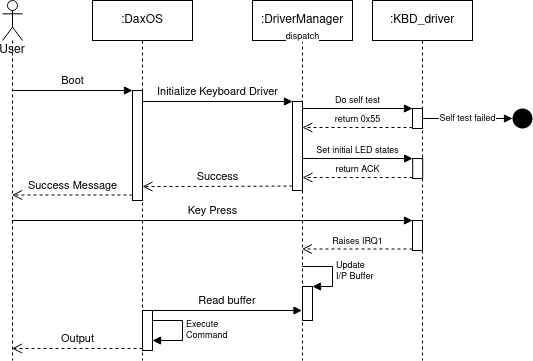
\includegraphics[width=\textwidth,height=\textheight,keepaspectratio]{kbd_driver}
	\caption{Sequence Diagram for keyboard driver}
\end{figure}
\pagebreak


\subsection{User Command}
\begin{flushleft}
	After boot the user interacts with DaxOS through a command prompt like windows. It
	is here that the user enters commands which will be executed by the kernel. These
	are not processes.
	
	Here the following commands are implemented:
	\begin{enumerate}
	\item \textbf{gfx\_demo}\\
	This demo program will demonstrate some of the graphics and drawing capabilities.
	\item \textbf{dcalc}\\
	This is a calculator application that can evaluate mathematical expressions.
	\item \textbf{term\_art}\\
	This will demonstrate some ASCII terminal art using VGA driver.
	\end{enumerate}

	The sequence diagram illustrates the process of running the commands. All the
	commands use operations from standard C library.To take input and output text to
	the screen the stdio functionality will be used.Then the command proceeds to do its
	computation. If dynamic memory is needed, the command again uses the malloc
	function from standard C library. The malloc function maintains a list of free stores -
	that is free blocks of memory. If the requested chunk of memory is already in the free
	store then the malloc function marks it as being used and returns a pointer to it. On
	the other hand if the memory in the list is not enough, the malloc function asks the
	kernel to provide more memory. In this case the kernel provides a new page
	to the malloc function and the malloc function promptly adds the block of memory
	into its free store and returns a pointer to it.
	
\end{flushleft}

\begin{figure}[h!]
	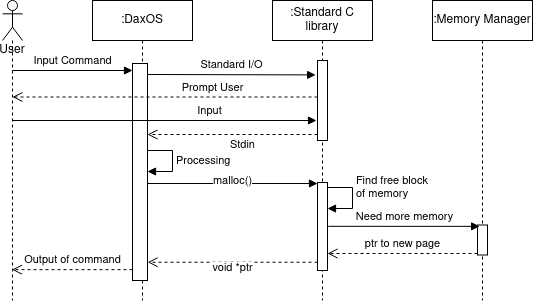
\includegraphics[width=\textwidth,height=\textheight,keepaspectratio]{user_command}
	\caption{Sequence Diagram for user command}
\end{figure}

\pagebreak
\subsection{Shutdown}
\begin{flushleft}
	Shutdown is implemented using Advanced Power Management (APM).\\
	Once the user initiates the shutdown command, there is no longer any interaction 
	between the user and the OS. The OS will request the power management module to perform the APC shutdown procedure.\\
	This involves calling a BIOS interrupt. This further requires switching from protected mode to real mode. 
	Once in real mode, the BIOS is informed about the kind of operation that needs to be performed.
	The BIOS is informed that it is required to perform APC operation by setting the
	register AX with the value 0x5307. The BIOS is informed that the current operation is to be done on all connected
	devices by setting register BX with the value 0x0001. Lastly the value 0x03 is put in the CX register to indicate shutdown
	operation. Now the BIOS function is activated by raising software interrupt 0x15.
	The computer is powered off.
\end{flushleft}
\vspace{1.5 cm}
\begin{figure}[h!]
	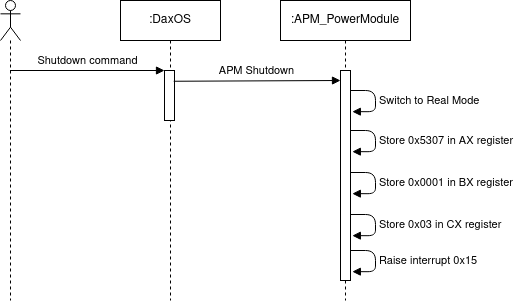
\includegraphics[width=\textwidth,height=\textheight,keepaspectratio]{shutdown}
	\caption{Sequence Diagram for system shutdown}
\end{figure}
% !TeX spellcheck = en_GB
\graphicspath{ {./diagrams/} }
\chapter{Other Design Considerations}\label{chapter:Other Design Considerations}

\section{Kernel Architecture}

\begin{flushleft}
	There are three types of kernel architectures:
		\begin{enumerate}
			\item \textbf{Micro Kernel}
			\item \textbf{Monolithic Kernel}
			\item \textbf{Hybrid Kernel}
		\end{enumerate}
	
	This classification is based on what is in kernel space and what is in user space. There are four
	protection rings that represent the access a piece of software has to the hardware and system. Out
	of these only two rings are of interest:
		\begin{enumerate}
			\item \textbf{Ring 0}\\
			Code running in Ring 0 is said to be in supervisor mode. It has complete access to the hardware
			and system.
			
			\item \textbf{Ring 3}\\
			Code running in Ring 3 is said to be in user space. It has no direct access to hardware or the
			system. Instead it accesses the system through syscalls.
		\end{enumerate}
	These protections are not simply implemented by the Operating system. Instead they are a part of
	the CPU architecture. They are activated by asm code.
	\begin{itemize}
		\item In a \textbf{micro kernel} very limited amount of code is is in kernel space. For example, most drivers are
		in userspace.
		\item In a \textbf{monolithic kernel} device drivers and other similar modules operate in kernel space.
		\item A \textbf{hybrid kernel} is somewhere in the middle of what runs in kernel space and user space.
	\end{itemize}

	Dax OS has a monolithic design. This is motivated by two facts which are:
	\begin{itemize}
		\item The Linux kernel is monolithic. Therefore if we use a micro kernel architecture, students will not be
		able to transfer the knowledge that they acquired from our project into the linux development space.
		
		\item Our kernel operates completely in ring-0 i.e without any restrictions. Implementing user-mode
		is unnecessary since we have no user-mode programs. Additionally students need to be in ring-0
		to understand how the hardware works.
		
	\end{itemize}
	
\end{flushleft}
\begin{figure}[h!]
	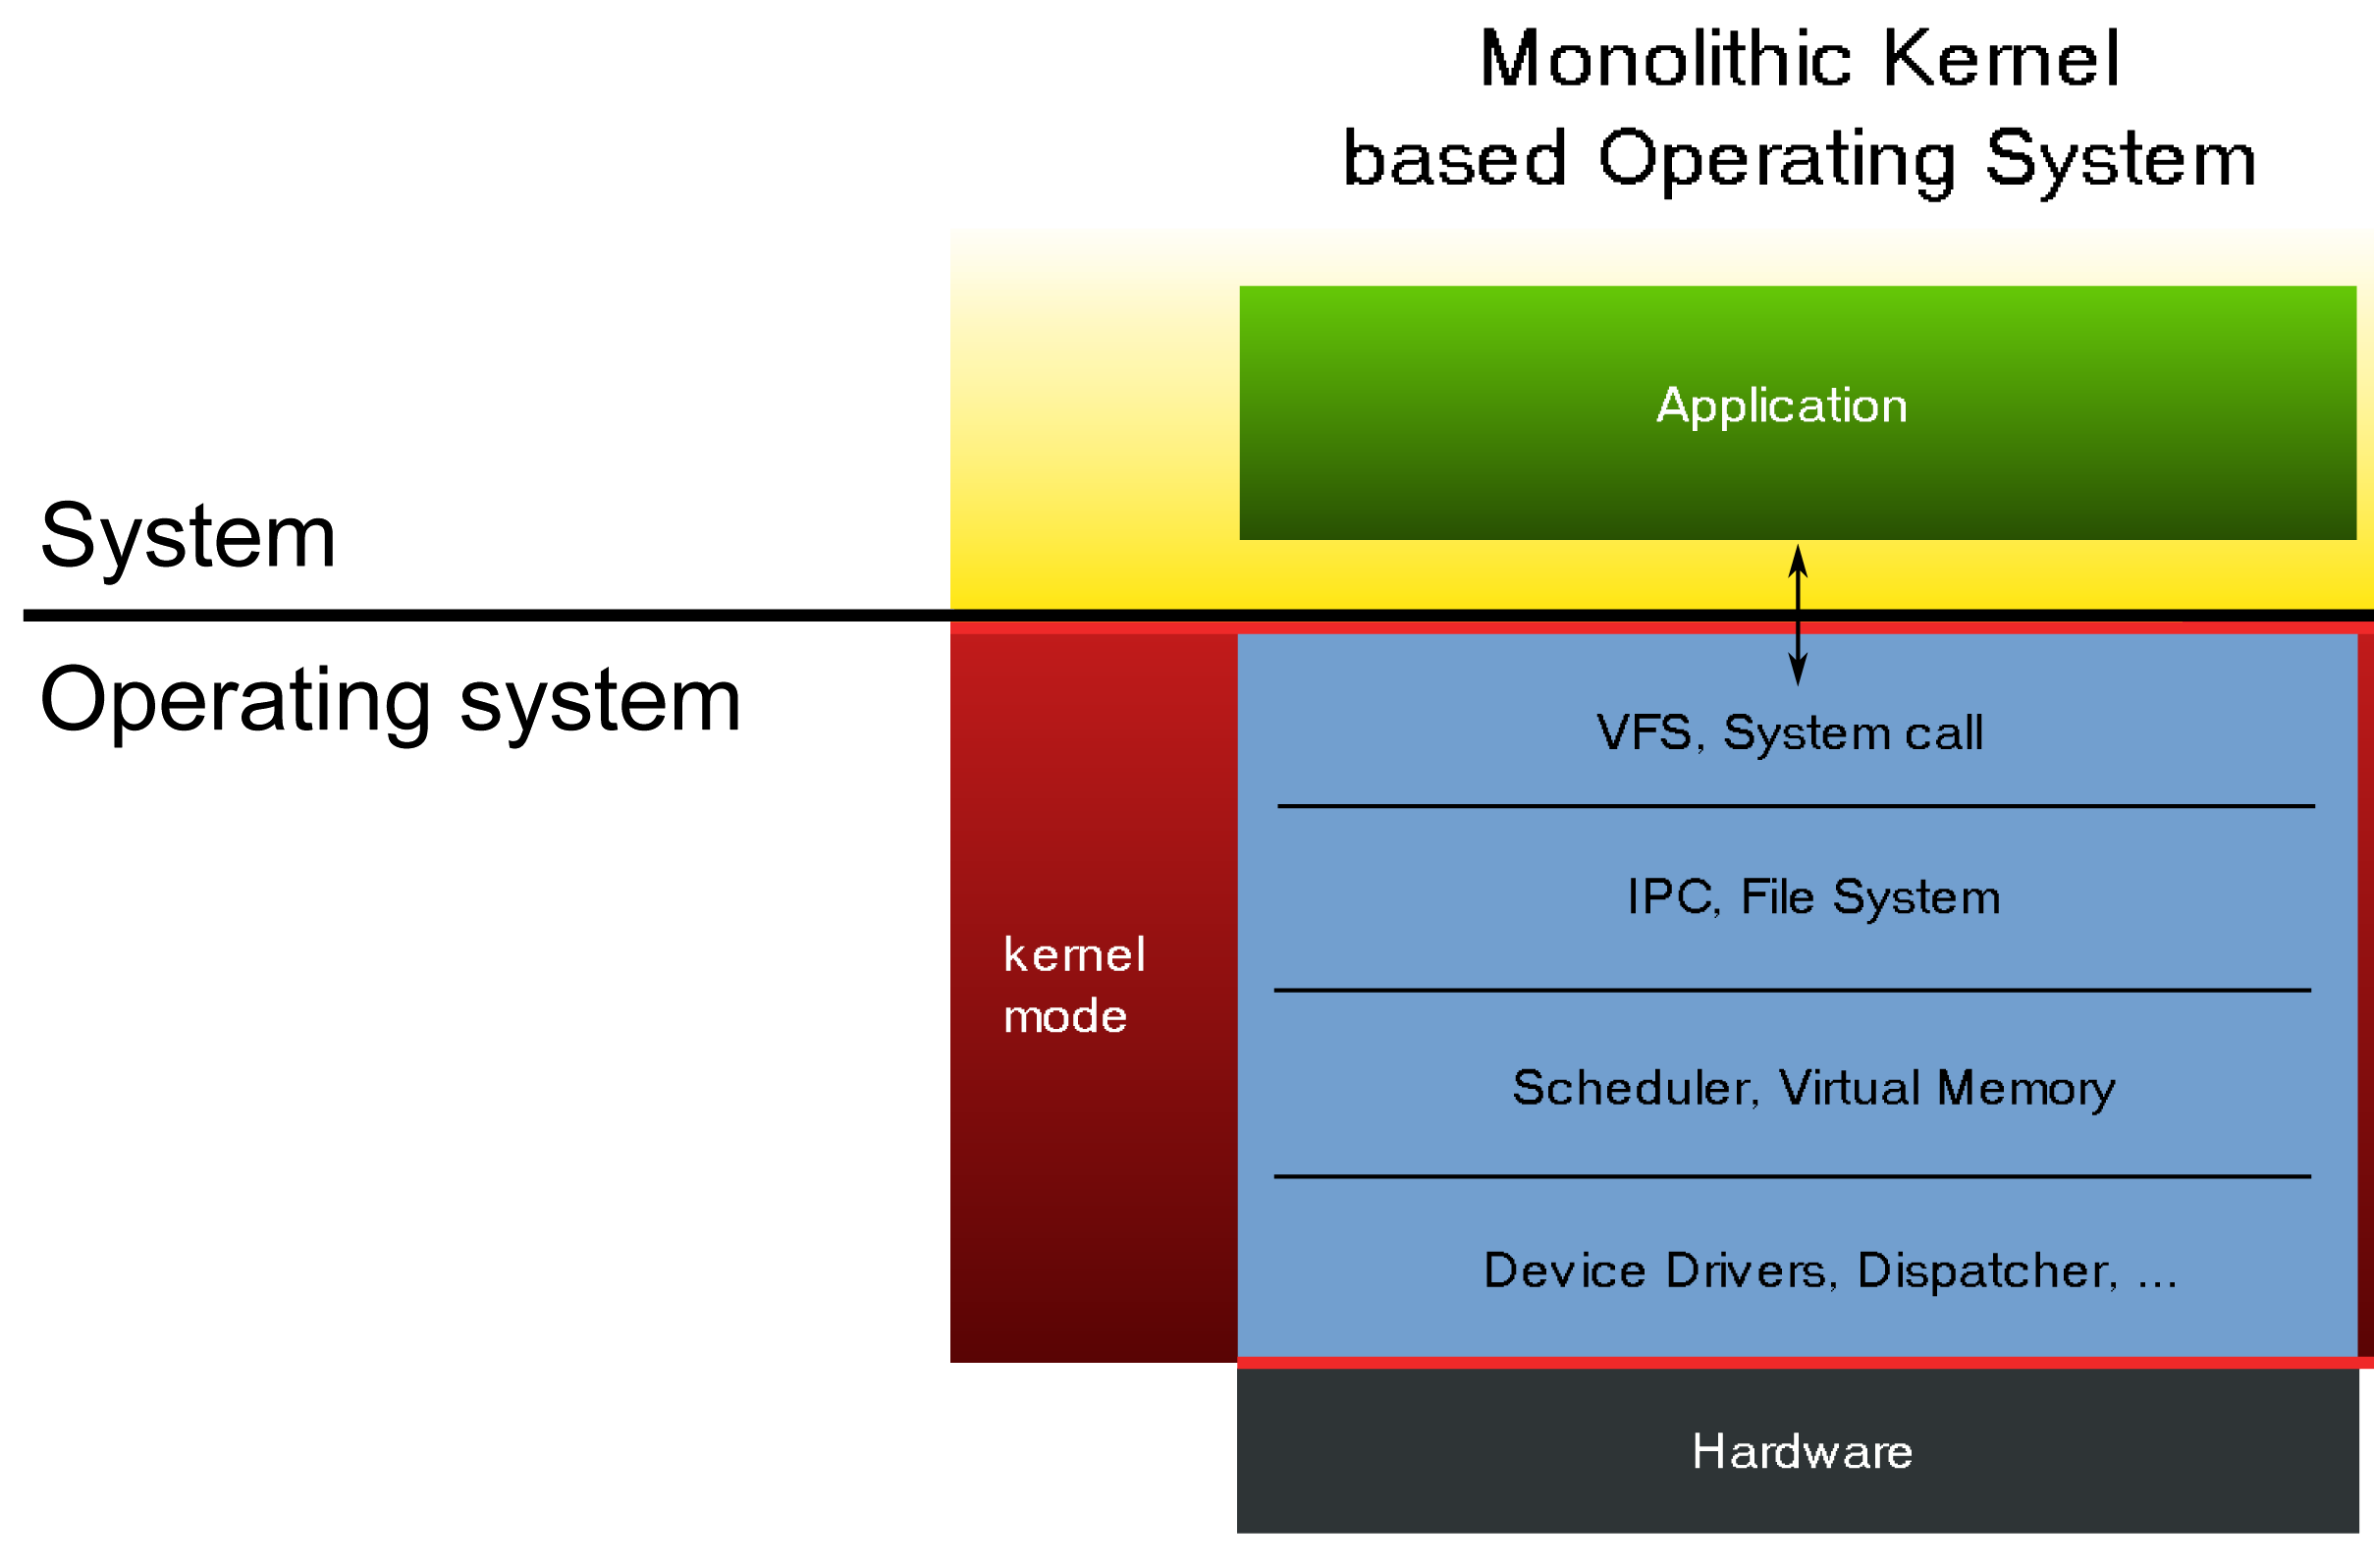
\includegraphics[width=\textwidth,height=\textheight,keepaspectratio]{kernel_arch}
	\caption{Illustration of Kernel Architecture}
\end{figure}
\pagebreak

\section{Build Process}
\begin{flushleft}
	The build architecture is a little involved because the C programming language
	does not have any real tooling for package management. Instead compiling and linking
	each translation unit must be done manually.
	\vspace{1.5 cm}
	
	A tool called GNU Make is used to manage the compilation process. GNU Make is a tool which
	controls the generation of executables and other non-source files of a program from the
	program's source files. It does this by executing commands in a file called Makefile.
	The makefile contains rules which specify what prerequisites are needed to build a particular
	executable and the steps required to build it. We have multiple Makefiles in this project to
	recursively compile and build each of our kernel components. In fact, the Makefiles by
	themselves account for 25\% of the codebase.
	\vspace{1.5 cm}
	
	The Makefiles are executed by issuing corresponding make commands (for eg: \textbf{make install} or
	\textbf{make install headers}). Shell scripts are being used to drive the make program. There is a shell
	script called config.sh that sets up the system environment variables that are utilized by make.
	The compilation process installs the operating system into the system root directory. This is currently the directory \textbf{sysroot} within the
	project. Sysroot directory further contains two sub-directories - boot and usr.
	The boot directory contains \textbf{DaxOS.kernel} file and the usr directory contains the standard C
	library and unit tests. The kernel is booted by pointing the bootloader to the /boot directory.
	The built kernel is tested on qemu by calling the qemu.sh shell script. This works by first
	packaging the kernel into a .iso image file and running qemu with the iso file.
	
\end{flushleft}
\pagebreak

\section{Keyboard Design Decisions}
\begin{flushleft}
	There are two design choices for the implementation of the keyboard driver:
	\begin{enumerate}
		\item \textbf{Polling Driven}\\
		In polling, the CPU keeps checking the status of PS/2 keyboard constantly to detect a keypress. The command-ready bit indicates that the 
		device needs servicing. This approach will lead to unnecessary loss of CPU cycles.
		\item \textbf{Interrupt Driven} \\
		When the user presses a key, the keyboard driver generates an interrupt which causes the CPU to run and ISR that handles the keypress.
		Interrupts are signalled by the interrupt request line.	
	\end{enumerate}
Interrupt driven implementation is more efficient than polling driven keyboard drivers.
Therefore interrupt driven keyboard drive will be implemented .The USB keyboard will be
supported by emulation.

\end{flushleft}

\section{Memory Segmentation}
\begin{flushleft}
	Segmentation involves splitting the available memory into segments each having a particular purpose. For example, code may be stored in the Code Segment and data may be stored in the data segment. In real mode, the memory address is of the form S:O where S denotes the segment and O is the offest within that segment. This virtual memory address is converted to physical memory address using the following equation:
	\[Physical Address = (S * 0x10) + O\]
	
	In 32-bit protected mode, segmentation is different in that it uses an entry in a table called GDT(Global Descriptor Table) instead of a segment number.
	Segmentation can be used to provide memory protection by controlling the memory access permission of each segment. 
	
	However, the use of segmentation to provide memory protection is often discouraged. For instance, you cannot use the C programming language if you use segmentation for memory protection as most C compilers do not support it. Therefore DaxOS does not use segmentation for memory protection. 
	
	Segmentation cannot be disabled but we can nullify the effects of segmentation by creating a flat memory model i.e we allow the the CS and DS to overlap and extend across all the available memory. This is practically accomplished by adding two entries in the GDT - one for the CS and another for DS. 
\end{flushleft}
%-----include as many chapters as needed-----%

\chapter{Conclusion}\label{chapter:Conclusion}
\begin{flushleft}
	This report has attempted to provide a sufficient and elaborate introduction to DaxOS.\\
	The implementation has been discussed along with code samples where applicable.		
	The authors of this report hope that the explanations were clear and succinct.
	\vspace{1.5 cm}

	Interested readers can find the source code of this project at \url{https://github.com/DaxKernel/OS}.\\
	You can also check out our website at \url{https://daxkernel.github.io/}.
\end{flushleft}

%%%-----BIBLIOGRAPHY-----%
%\addcontentsline{toc}{section}{REFERENCES}
%\bibliography{myreference}
%\bibliographystyle{IEEEtran}
%-----BIBLIOGRAPHY-----%
\cleardoublepage

\addcontentsline{toc}{chapter}{REFERENCES}
\begin{thebibliography}{99}
		\bibitem{1} https://wiki.osdev.org/Bare\_Bones
		\bibitem{2} http://www.osdever.net/tutorials/
		\bibitem{3} https://wiki.osdev.org/Interrupts\_tutorial
		\bibitem{4} https://wiki.osdev.org/User:Omarrx024/VESA\_Tutorial
		\bibitem{6} https://wiki.osdev.org/Exceptions
		\bibitem{7} https://wiki.osdev.org/Scalable\_Screen\_Font
		\bibitem{8} https://wiki.osdev.org/PS/2\_Keyboard
		\bibitem{9} https://www.gnu.org/software/grub/manual/multiboot/multiboot.html
	\end{thebibliography}

\end{document}  % document ending 

%To run, go to the directory where the files are saved, and type:'latex FILENAME.tex' 
%To generate the PDF, type: 'dvipdfm FILENAME.dvi' 
%To generate the References page, type the following commands: 
%'latex FILENAME.tex' 
%'bibtex FILENAME.aux' 
%'latex FILENAME.tex' 
%'latex FILENAME.tex' 
%'dvipdfm FILENAME.dvi' 

